\documentclass[conference]{IEEEtran}

\usepackage[cmex10]{amsmath}
\usepackage{xcolor}

\usepackage{graphicx}
\hyphenation{op-tical net-works semi-conduc-tor}


\begin{document}
\title{Week 1 Report\\ECE 432 Microwave Circuit Design II}

\author{\IEEEauthorblockN{Jackson Pugh}
\IEEEauthorblockA{Portland State University\\
Portland, OR 97207\\
Email: japugh@pdx.edu}
\and
\IEEEauthorblockN{Michael Woodruff}
\IEEEauthorblockA{Portland State University\\
Portland, OR 97207\\
Email: michael.woodruff@pdx.edu}}
\maketitle


\begin{abstract}
%\boldmath
A quadrature hybrid coupler circuit will be designed and simulated in ADS and built and tested in the lab.  The overall theory is discussed in Chapter 7 of the David Pozar textbook.  The results obtained from the lab successfully matched the expected theory of operation for the quadrature circuit.
\end{abstract}
\IEEEpeerreviewmaketitle


\section{Introduction}
This lab involves designing and building a quadrature circuit to operate at 1 GHz with the standard 50 $\Omega$ impedances.  The following section walks through the design process.
\section{Design Approach}
The reference design for the quadrature circuit was taken from \cite{IEEEhowto:kopka}.  From this template, the characteristic impedance for each side and the wavelength was determined for a designed cutoff of 1 GHz.  Table~\ref{tab:layout} contains the values (see lab notebook for hand calculations).  Then an ideal and non-ideal quadrature circuit was designed and simulated in ADS.  The ideal circuit was made using the ideal TLIN and the non-ideal was made using the MLIN with an MSTUB populated with estimated values for the FR4 board that would be used in building and measuring the sticky tape layout.\\\\
After analyzing the simulation results for both circuits, the sticky tape board was designed and the measurements were taken for Port 2 and Port 3.  The data were saved as S2P files and then imported into ADS for comparison with the circuit simulation.  The following section answers questions and provides insight on specific topics in the design process.  Analysis on the lab measurements and simulation results are given at the end.
\section{Questions \& Answers}
1. Sketch the layout of your component; start with an idealized case and indicate electrical lengths and characteristic impedances of the lines. Then construct what the realistic layout may look like. If needed, you may want to use some "mitered" and/or meandering lines to fit your circuit inside the given PCB.\\\\\\
\textcolor{red}{For the quadrature circuit, only the width and length for the circuit are adjustable; there are no comopnents.  Table~\ref{tab:layout} contains the electrical length and characteristic impedance of the lines for the quadrature circuit.  Figure~\ref{fig:pozar_hybrid} shows the ideal quadrature circuit layout.  Figure~\ref{fig:ads_layout} shows the realistic layout.\\\\
Note: There are sharp edges in the realistic circuit which may produce EMI radiation and cause unwanted sources of noise in the signal.  Mitering these corners would be advisable to reduce EMI.}\\\\
\begin{table}[!h]
    \centering
    \caption{Ideal Impedance and Length}
    \begin{tabular}{|l|l|}
    
        \hline
        Parameter                         & Value  \\ \hline
        Characteristic Impedance ($\Omega$) & 50     \\  \hline
        Wavelength $\lambda$ (m)          & 0.1676 \\
        \hline
    \end{tabular}
\label{tab:layout}
\end{table}

\begin{figure}[!h]
\centering
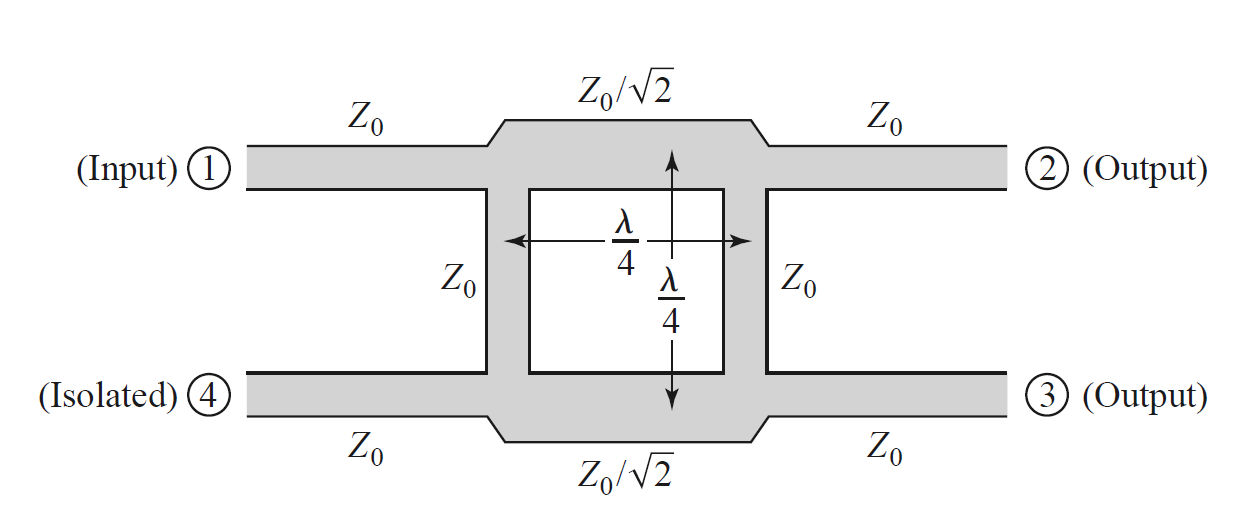
\includegraphics[scale=0.25]{pozar-hybrid.png}
\caption{Hybrid Quadrature Geometry Circuit Layout (image from Pozar)}
\label{fig:pozar_hybrid}
\end{figure}

\begin{figure}[!htb]
\centering
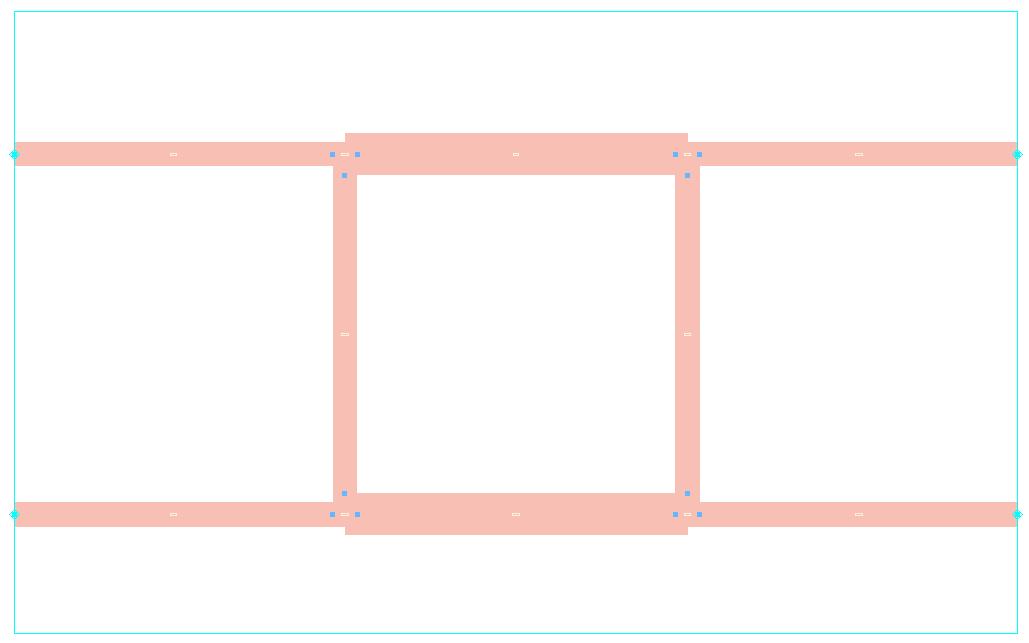
\includegraphics[scale=0.25]{ads-layout.png}
\caption{ADS Quadrature Circuit Layout}
\label{fig:ads_layout}
\end{figure}
% Question 2
2. Implement your idea in ADS using idealized microstip components. (You can go to different levels of accuracy by, for example, utilizing T-junctionsto connect lines of different lengths. If you need meanders you may also want to use mitered corners.)\\\\\\
\textcolor{red}{ Figure~\ref{fig:ideal_circuit} shows the ideal quadrature circuit in ADS.  Figure~\ref{fig:nonideal_circuit} shows the non-ideal quadrature circuit in ADS.}\\
\begin{figure}[!htb]
\centering
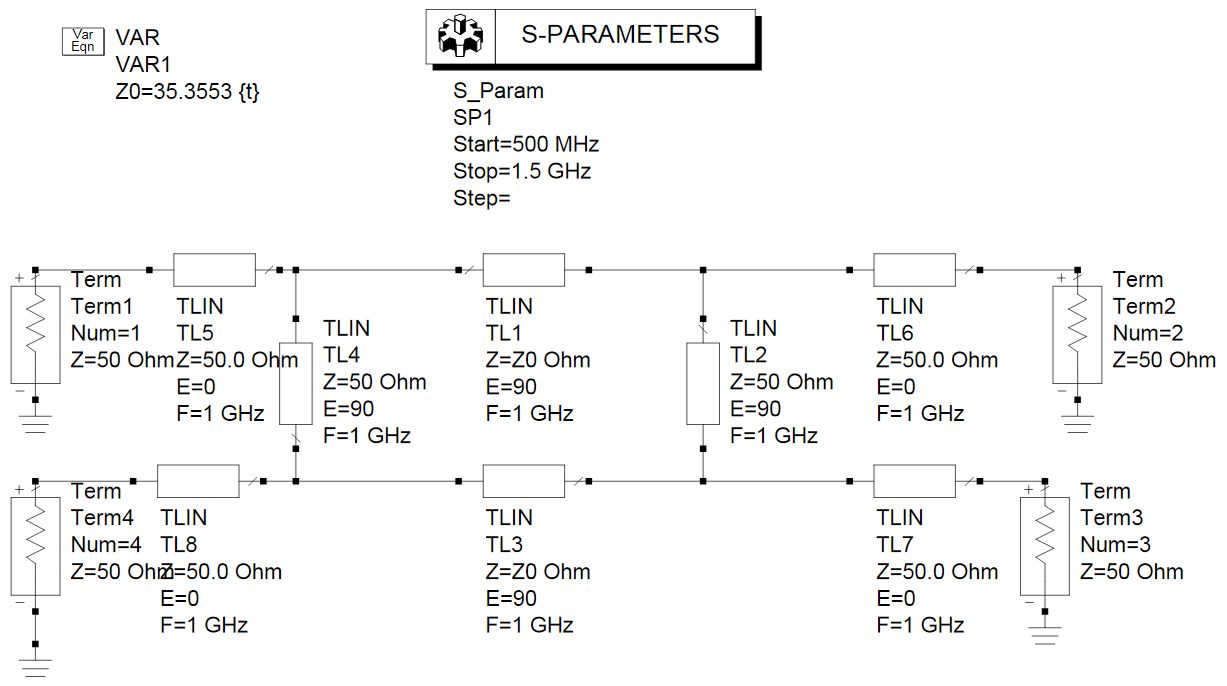
\includegraphics[scale=0.25]{quadrature-ideal-circuit.png}
\caption{Ideal Quadrature Circuit}
\label{fig:ideal_circuit}
\end{figure}
\begin{figure}[!htb]
\centering
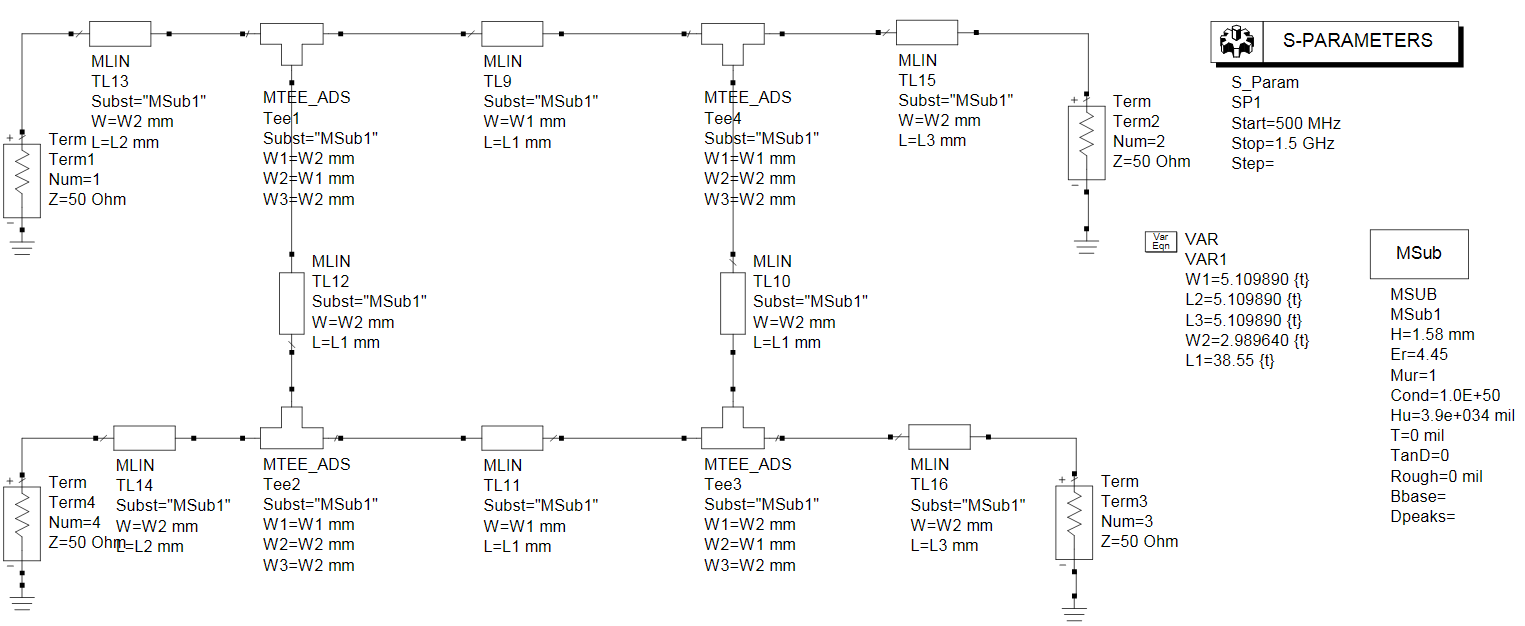
\includegraphics[scale=0.2]{quadrature-nonideal-circuit.png}
\caption{Non-Ideal Quadrature Circuit}
\label{fig:nonideal_circuit}
\end{figure}

% Question 3
3. Simulate the response of your circuit – make sure that you have the right number of ports, e.g. three ports for Wilkinson divider and four for the coupler.\\\\\\
\textcolor{red}{Figure~\ref{fig:ideal_plot} shows the simulation result for the ideal quadrature circuit.  Figure~\ref{fig:nonideal_plot} shows the simulation result for the non-ideal quadrature circuit.\\\\
Note: The main difference between the ideal and non-ideal quadrature circuit lies in the S11 (reflection coefficient) value at the cutoff frequency.  Ideally, there should be 0 reflection (i.e. S11 at the cutoff frequency should be -$\infty$ dB--this would indicate maximum power transfer).  The non-ideal circuit has the MSTUB parameters which accounts for partial power loss.  This results in the S11 signal being higher than the ideal circuit which uses ideal transmission lines.}\\

\begin{figure}[!h]
\centering
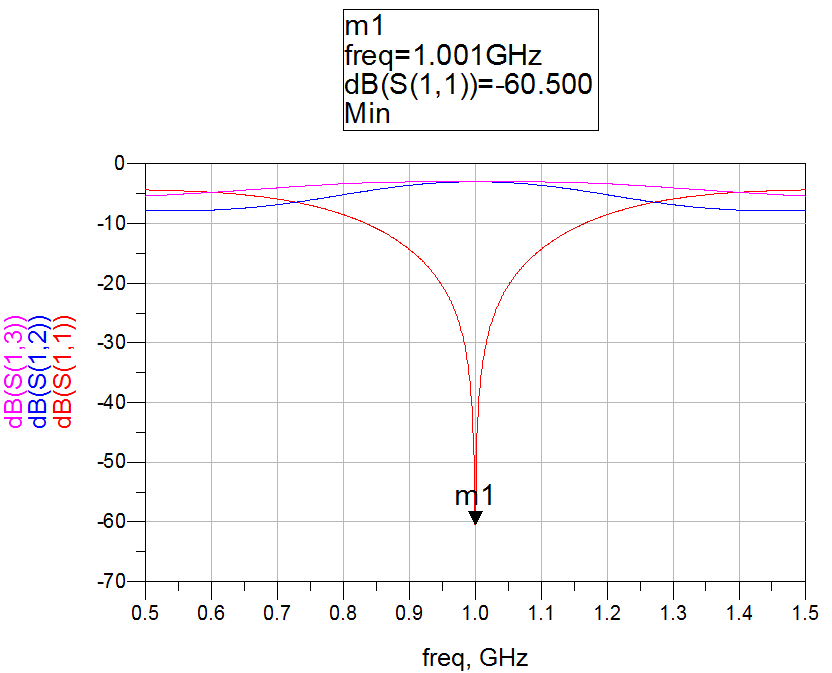
\includegraphics[scale=0.35]{quadrature-ideal-plot.png}
\caption{Ideal Quadrature Simulation Plot}
\label{fig:ideal_plot}
\end{figure}

\begin{figure}[!h]
\centering
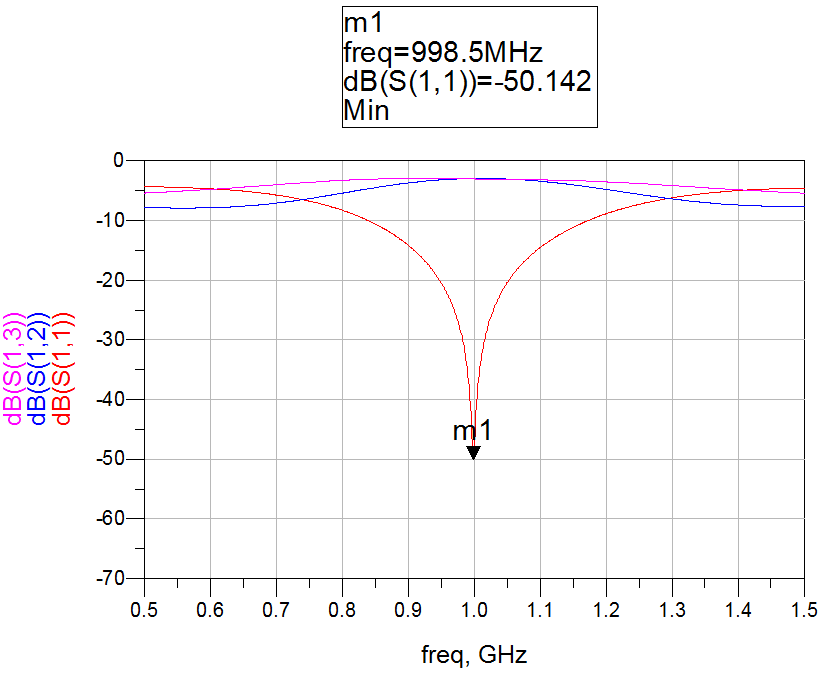
\includegraphics[scale=0.35]{quadrature-nonideal-plot.png}
\caption{Non-Ideal Quadrature Simulation Plot}
\label{fig:nonideal_plot}
\end{figure}

% Question 4
4. Q: comment on how close your simulation came to ideal expectations. Reproduce figure 7.12 from Pozar’s book (it shows "frequency response of an equal-split Wilkinson power divider") or figure 7.25 "Scattering parameter magnitudes versus frequency for the branch-line "coupler …"\\\\\\
\textcolor{red}{Figure~\ref{fig:pozar_plot} shows the image from Pozar.  The simulations for both the ideal and non-ideal quadrature circuits are close to Figure 7.25 from Pozar.}\\
\begin{figure}[!h]
\centering
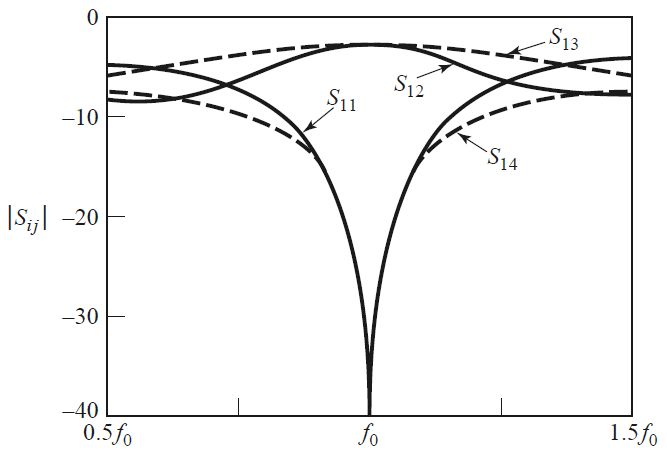
\includegraphics[scale=0.35]{pozar_plot.png}
\caption{Pozar Plot (See Figure 7.25)}
\label{fig:pozar_plot}
\end{figure}

% Question 5
5. Use the "tuning" feature of ADS to determine what happens as dimensions of lines (their electrical length and characteristic impedance change). Report your observations. Are some parameters more important than others? Explain. How would you do this systematically?\\\\
\textcolor{red}{As the characteristic impedance is changed, the amount of reflection (S11) decreases and the power transfer to Port 2 and Port 3 become unequal.  As the electrical length is changed, the cutoff frequency shifts--longer electrical length results in lower cutoff frequency and shorter electrical length results in higher cutoff frequency.}\\\\\\
% Question 6
6. Build your circuit; remember that you can measure only two ports. What are you going to do with the remaining port(s)?\\\\\\
\textcolor{red}{The unused port(s) must be terminated to ground using a 50 $\Omega$ resistor to match the transmission line.}\\

% Question 7
7. Include a photo of your circuit.\\\\\
\begin{figure}[!h]
\centering
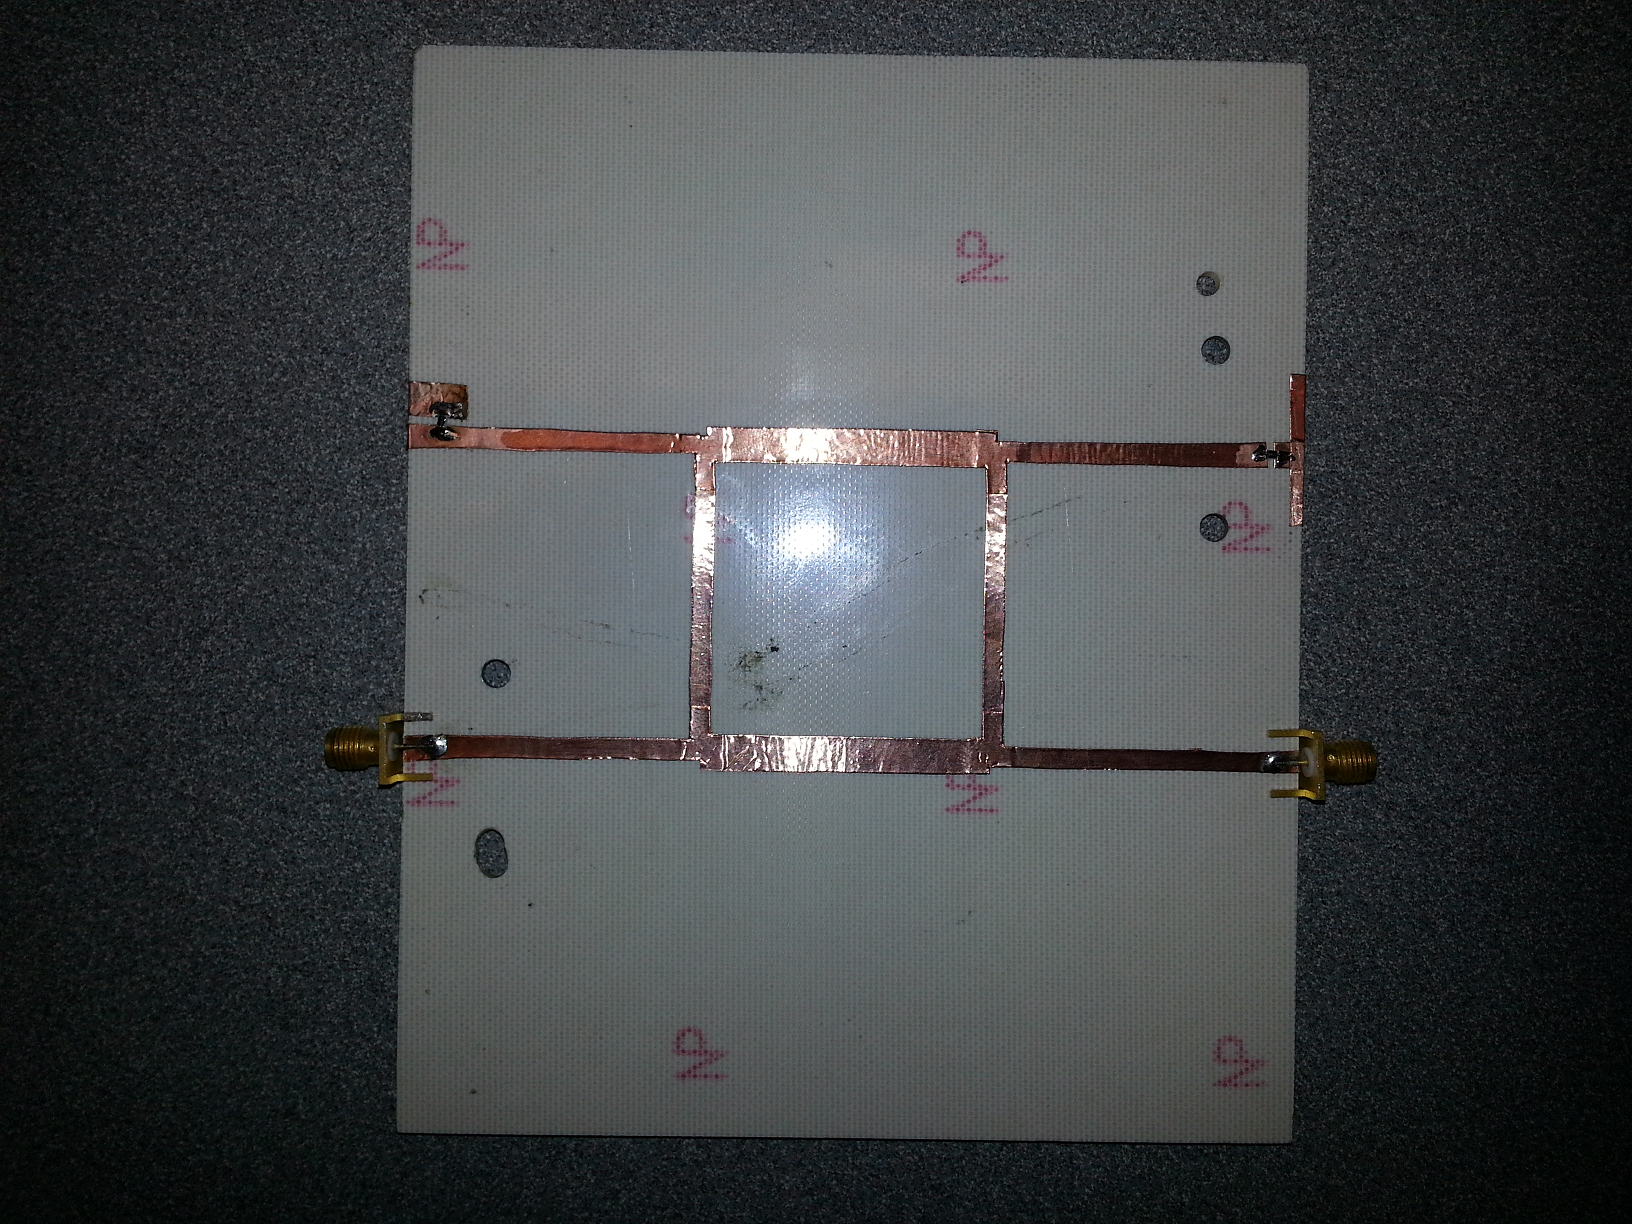
\includegraphics[scale=0.15]{quadrature-board.png}
\caption{Quadrature Board Screenshot}
\label{fig:board}
\end{figure}

% Question 8
8. Compare your measured and simulated results. Comment on how close they are and what may need to be fixed to get better agreement.\\\\\\
\textcolor{red}{Figure~\ref{fig:labdata_plot} shows the imported S2P data from the VNA plotted in ADS.}
\begin{figure}[!htb]
\centering
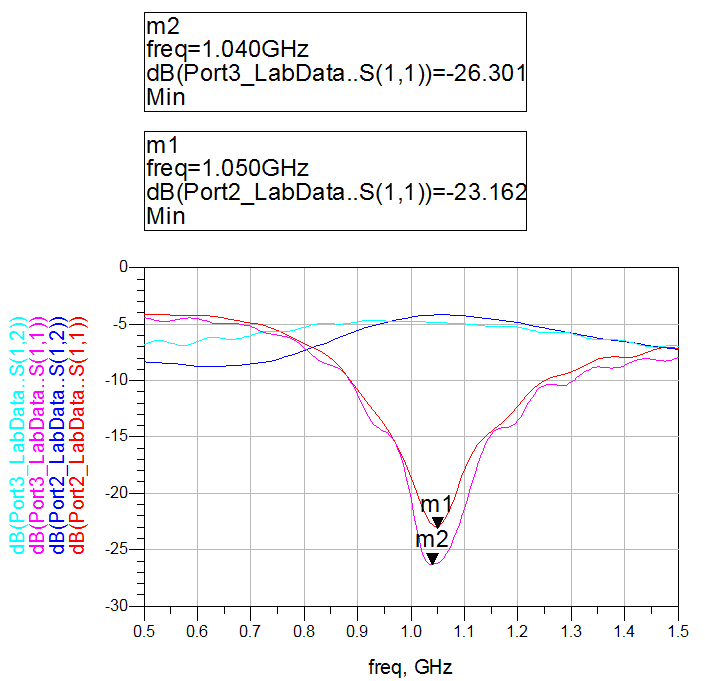
\includegraphics[scale=0.35]{quadrature-labdata-plot.png}
\caption{Quadrature Lab Data Plot}
\label{fig:labdata_plot}
\end{figure}

\textcolor{red}{There are many differences between the lab measurements and the ADS simulations.  These include the cutoff frequency at 1.04 GHz (instead of 1 GHz), wavy signals, lower S11 (reflection coefficient) attenuation, and uneven symmetry along the cutoff frequency.  These could be fixed by having more accurate widths and lengths for the transmission lines (the length determines where the cutoff frequency occurs--in this case, the length was too short thus pushing the cutoff frequency above 1 GHz).  In addition, the sharp edges on the layout probably caused the wavy lines so using some sort of mitigating technique mentioned earlier could reduce this.  Lastly, proper calibration can also have a significant effect when measuring data.  This may not have been done for the second port measurement (since there was a period of time when the SMA connector had to be desoldered and resoldered).  Overall, for a sticky-tape method the results are acceptable and shows the circuit functions as it should.}\\

% Question 9
9. If there is time, try to simulate the other component, following the procedure above.\\\\\\
\textcolor{red}{N/A}

\section{Weekly Lessons}
\subsection{In-Class}
ABCD Parameters \cite{abcd}: These network parameters are useful when analyzing cascaded two-port networks.  This is done through the process of matrix multiplication.  In general, for a lossless network, the following holds:
\begin{itemize}
\item A is real
\item B is imaginary
\item C is imaginary
\item D is real
\end{itemize}

\subsection{Outside of Class}
Fundamentals of Choosing LDO and Switching Regulator Webcast \cite{edn}:  The webcast discussed the parameters of the LDO including input/output voltage/current, input/output regulation, PSRR, fixed/adjustable output via jumper/resistor, operating frequency, footprint, noise figure, and packaging and heat sink options.  Other important points to consider are operating temperature range, themeral/overload/underload protection, and pricing/availability.  Then it highlighted the tradeoffs between the LDOs and switchers which included physical size, noise, EMI/RFI, beats, and efficiency (and at what load).  Ultimately, the decision for choosing a regulator depends on fully understanding the needs of the application and assigning priorities correctly.

%\section{Conclusion}
%The conclusion goes here.
\begin{thebibliography}{1}
\bibitem{IEEEhowto:kopka}
Pozar, David M. Microwave Engineering. Hoboken: Wiley \& Sons, 2011. Print.
\bibitem{abcd}
http://whites.sdsmt.edu/classes/ee481/notes/481Lecture20.pdf
\bibitem{edn}
http://www.techonline.com/electrical-engineers/education-training/courses/4410927/Fundamentals-of-Choosing-LDO-and-Switching-Regulators
\end{thebibliography}
\end{document}